


\chapter{State of the Art }%
\label{chap:StandderTechnik}%


Autonomous Vehicle software follows the sense-plan-act principle. Localization is part of the sense block, and is a crucial component for modern-day AVs \cite{goelles_fault_2020}. But research has shown a high degree of sensitivity in localization algorithms \cite{albrecht_investigation_2022}, which is why, in the following, the current state of the art with respect to mapping and localization algorithms, sensors, and their data needed and how that data degrades under adverse conditions, will be depicted. 

% \begin{figure}[htbp]
%     \centering
%     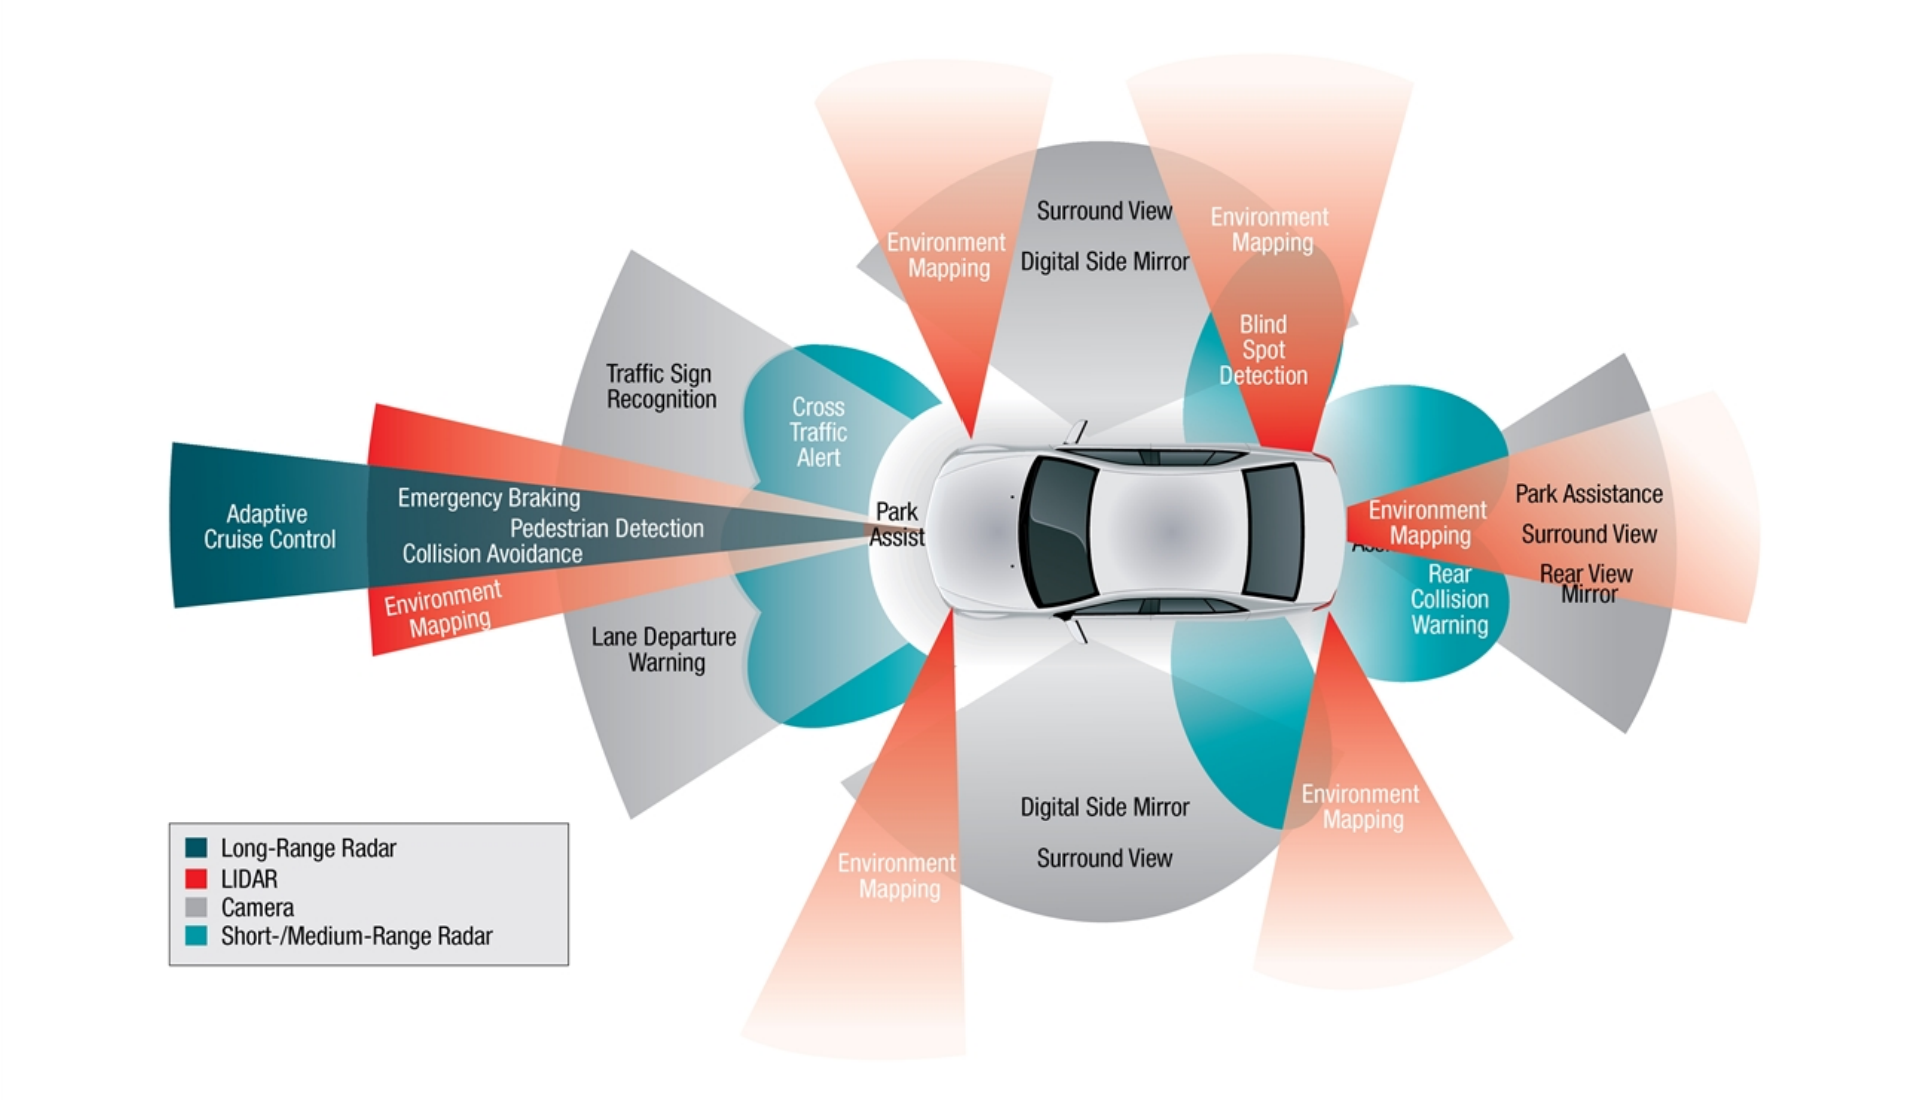
\includegraphics[scale=0.7]{figures/Figure_2__SensorsOnAV.png}
%     \caption{%
%     \textbf Schematic overview of the primary sensor modalities used in autonomous vehicles and their respective roles within the perception and localization pipeline. \cite{https://ieeexplore.ieee.org/stamp/stamp.jsp?tp=&arnumber=8398279}.
%     }
%     \label{fig:figure_1_2}
% \end{figure}

Currently, Level three AVs are available for purchase commercially, while Level four is still under development. To make level four AVs commercially available and eventually reach full autonomy with level five autonomy, we require a diverse portfolio of sensors. 

The perception block of Figure 1.2 can be broken down into mapping, localization, and detection. For this thesis, the detection aspect is not relevant and will not be discussed. It will focus on mapping and localization
\section{Positioning within the FTM Chair}
This Thesis support Karunaianayagam's research in localization safety. His research focuses on what happens if an automated driving system fails and how it could be managed. 

The first question, that needs to be answered is: Is a safe execution of the driving task possible? 
If this is not the case, then the system must enter a fail-degraded state. If this state is entered, the AV must come to a sage stop. This can be an emergency stop, a comfort stop or the vehicle can pull over.
It is important to asses which maneuver is the least risky. At Levels 4 and 5, the ADS can automatically achieve the minimal risk condition by performing the DDT fallback. Alternatively, if the Level 4 or 5 vehicle is also designed to accommodate operation by a driver, it may also allow the user to perform the DDT fallback. 


This maneuver is known as a Minimum Risk Maneuver (MRM). Within the autonomous driving stack, the Dynamic Driving Task (DDT) comprises the operational and tactical actions carried out by the Automated Driving System (ADS), including the execution of an MRM when system limits are encountered. Upon successful completion of an MRM, the vehicle transitions into a Minimum Risk Condition (MRC), which represents a state in which the vehicle can either remain stationary or safely transfer driving responsibility back to the human driver.

In SAE Level 3 systems, the ADS cannot guarantee autonomous attainment of the MRC under all operating conditions, as a timely intervention by the human driver may be required. This limitation constitutes a fundamental distinction between Level 3 and Level 4/5 automation and presents a significant challenge for current autonomous driving research.

In order to evaluate these maneuvers and the ADS reaction to edge cases, without performing expensive real-life tests, this thesis aims to create a fault injection tool, which can then be used to generate adverse weather scenarios to stress test ADS's. These scenarios can also be used for other applications such as object detection. 

A schematic illustration of how this thesis will supplement localization algorithms and how the impact of the faults on the localization will be measured can be found in 

%%%%NIJI PRESENTATION CITATION%%%%

\begin{figure}[htbp]
    \centering
    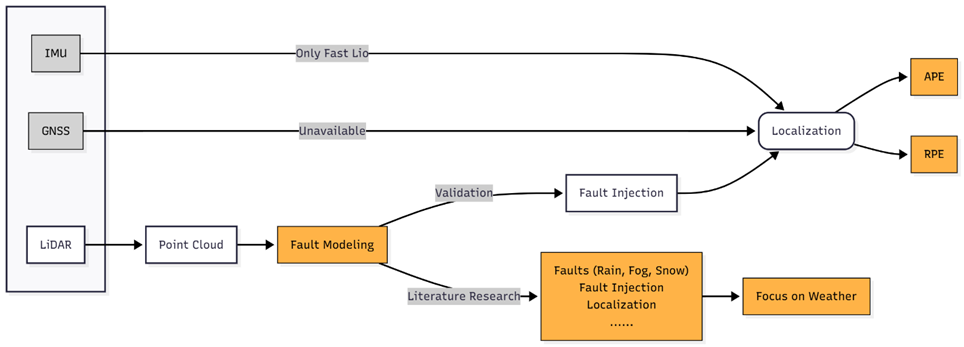
\includegraphics[scale=1]{figures/Figure_2_1_Einordnung.png}
    \caption{%
    \textbf Thematic classification of thesis topic, highlighting direct contributions in orange \cite{}.
    }
    \label{fig:figure_1_2}
\end{figure}

\section{Sensors}

\subsection{Overview}
Sensors provide the lense through which the autonomous vehicle perceives its surroundings. This means that the entire perception pipeline, including object detection and classification, localization, as well as mapping, is based on input generated from sensors. In modern cars, implementing redundancy, often through duplication or even triplication \cite{matos_survey_2024} %4.5% 
, is crucial. 
This mean, that car manufacturers install multiple of the same components, which all have the same function. 

For instance, BMW's autonomous driving system installs three different AD (Autonomous Driving) channels \cite{furst_scalable_nodate}.



The most important and commonly used sensors for perception in AVs are: 
\begin{itemize}
    \item LiDAR (Light Detection and Ranging): 
    \item Camera
    \item RADAR (Radio Detection and Ranging)
    \item GNSS (Global Navigation Satelite System)
    \item Inertial Measuring Unit 
    \item Ultrasonic 
\end{itemize}

A brief illustration of each sensor's characteristics can be found in Figure 2.3.  





\begin{figure}[htbp]
    \centering
    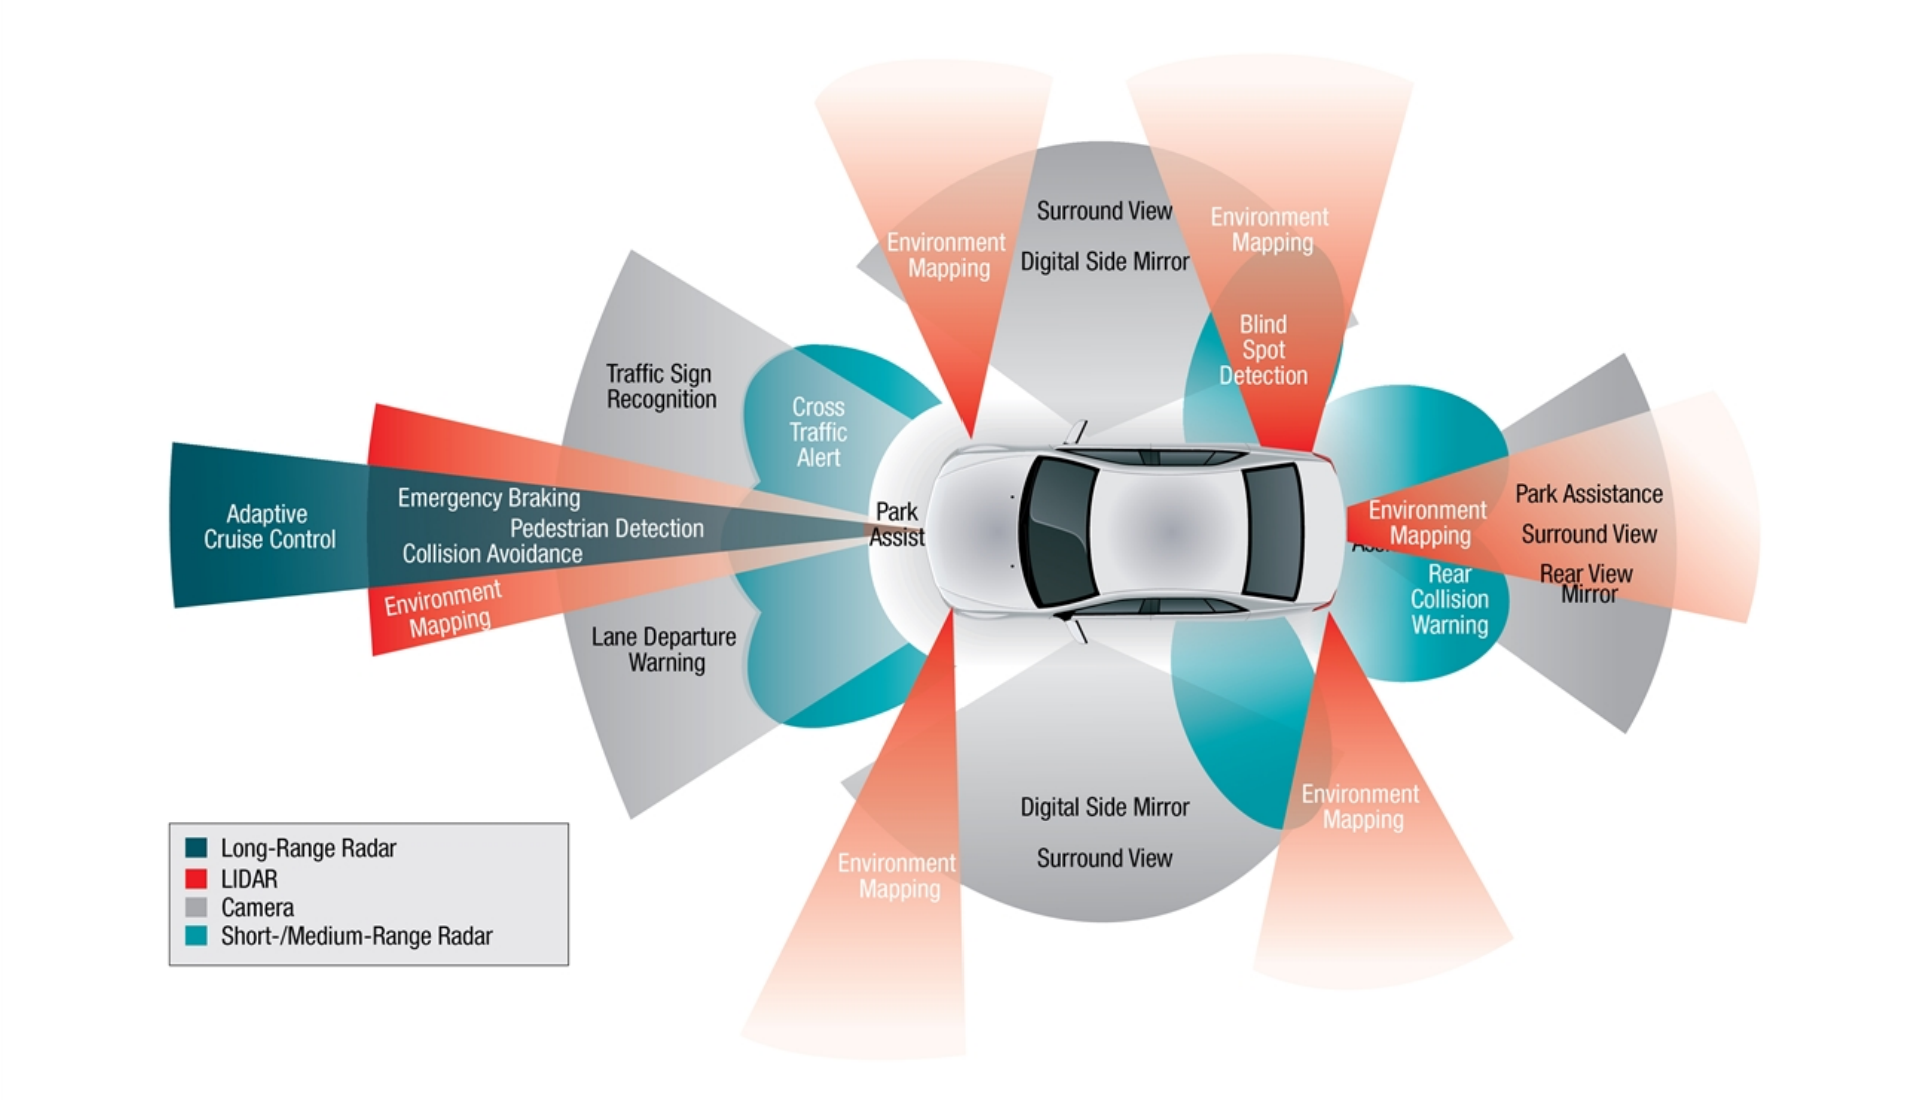
\includegraphics[scale=0.7]{figures/Figure_2__SensorsOnAV.png}
    \caption{%
    \textbf{Schematic overview of the primary sensor modalities used in autonomous vehicles and their respective roles within the perception and localization pipeline. \cite{taraba_utilization_2018}
    }}
    \label{fig:figure_1_2}
\end{figure} 

Cameras are mostly used for object detection, classification, and semantic understanding of the driving scene. Cameras have the advantage, that the entire traffic infrastructure, such as lane markings or traffic signs, is inherently visual. Cameras offer great contextual information, spatial resolution, and aren't particularly costly. But as it is a passive sensor, it cant measure depth or relative velocity accurate. This results in Cameras being limited in their ability to perform precise localization and mapping. 

In contrast, RADAR is an active sensor, and can measure depth and velocity accurately through Doppler measurements. It holds its accuracy over long distances and is therefor a good option for cruise control or brake assistance systems. 
Due to its low angular resolution it cannot produce detailed spatial representations of its enviornments, which also makes this sensor unsuitable for localization algorithms. 

GNSS provides global position estimates and is commonly used as a localization reference. However, its accuracy degrades significantly in urban environments due to multipath effects, signal occlusions, and atmospheric disturbances. Consequently, GNSS alone is insufficient for reliable localization in dense traffic scenarios and complex urban settings

%CITE JOHANNES BETT LECTURE 

For localization and mapping LiDAR is the most important sensor, since it is an active sensor with a good angular resolution. Something all of the other sensors lack.
Its ability to accurately detect depth as well as the velocity of objects in its surroundings makes it very capable for mapping, and therefore it will be the sensor this thesis will work with. 

However, a significant drawback of LiDAR sensors is its vulnerability to weather effects, which highlights the need for research in the field of weather effects on LiDAR.  
%%%ADD JOHANNES BETZ CITATION HERE%%%%


\subsection{LiDAR}

LiDAR (Light Detection and Ranging) is an active sensing technology originally developed in the 1970s for space platforms. Similar to RADAR, LiDAR systems operate based on the time-of-flight (ToF) principle. A laser diode emits a short pulse of light in the infrared spectrum, which is reflected by objects in the environment and subsequently detected by the system’s receiver.

The LiDAR system emits a laser pulse with a finite duration $\tau$ and simultaneously triggers an internal timing circuit. When the reflected pulse is detected by the photodetector, an electrical signal is generated that terminates the timing process~\cite{vargas_overview_2021}.  

Using the measured round-trip ToF $\Delta t$, the distance to the reflecting object can be computed. This measurement principle is illustrated in Figure~2.4 and formalized in Equation~(1).

\begin{figure}[htbp]
    \centering
    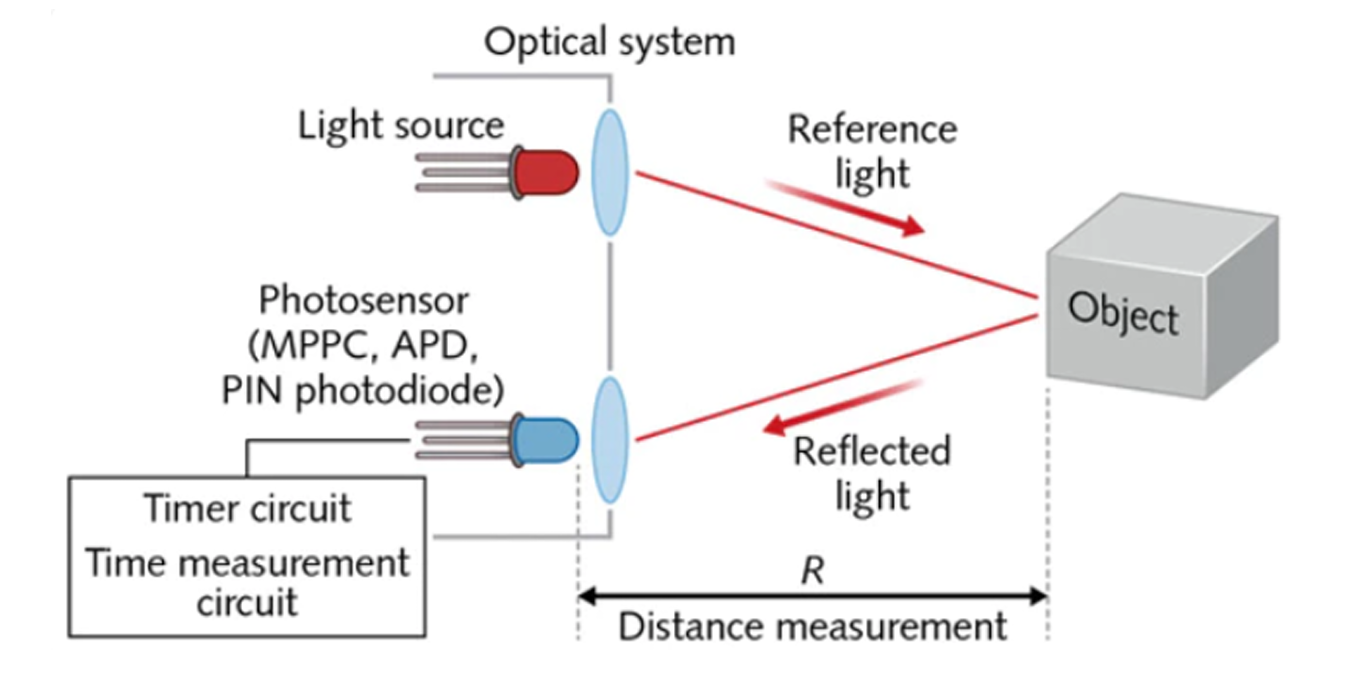
\includegraphics[scale=0.7]{figures/LiDAR_Picture.png}
    \caption{%
    \textbf{Schematic overview of the operational principle of a LiDAR system}~\cite{li_lidar_2017}.
    }
    \label{fig:figure_1_2}
\end{figure}

\begin{equation}
R = \frac{c \, \Delta t}{2n}
\end{equation}

Here, $R$ denotes the estimated distance to the target, $c$ is the speed of light, and $n$ represents the refractive index of the propagation medium, which can be approximated as $n \approx 1$ for air. The time-of-flight $\Delta t$ is measured independently for each point by the LiDAR sensor~\cite{li_lidar_2017}.

The power detected by the photodetector can be calculated using Equation~(2). 

\begin{equation}
\label{2}
P(R) =
P_0 \,
\frac{\rho \, A_0}{\pi R^2} \mu_0
\, \exp\!\left(-2 \gamma R\right)
\end{equation}

In this equation, $P_0$ is the peak power of the laser pulse, $\rho$ is the targets reflectivity, $A_0$ is the receiver's aperture area, $\mu_0$ is the spectral transmission of the detectiono optics, $\gamma$ is the atmospheric extinction coefficient and c as well as n were explained in Equation~(1) \cite{vargas_overview_2021}.

Each point is retained if the power received by the photodetector exceeds the threshold power %%%%FIND SOURCE AND CITE%%%%%. 
It then creates a three-dimensional point cloud of its surroundings and usually has about 20 degrees in elevation \cite{vargas_overview_2021}


\section{Relevant LiDAR Point Cloud Faults }
In order to understand what issues LiDAR point cloud faults cause and to analyze the point cloud defects, it is important to understand which faults are relevant to this discussion. 

Faults can occur on various levels of an automotive perception system. It could be the sensor fusion layer, an individual sensor and its components or the entire perception system \cite{FDIIR}. 
Since this a broad range of faults, they can be classified into the following categories: defect suncomponent, mechanical damage to sensor cover, layer on sensor, mounting issue, security attack, unfavourable enviornmental condition , and crosstalk \cite{goelles_fault_2020}. These are highlighted in table 1.

%Table 2.1
\begin{table}[htbp]
\centering
\caption{Classification of perception sensor faults including exemplary faults and related international safety standards.}
\label{tab:sensor_faults}
\begin{tabular}{|p{4cm}|p{6cm}|p{3cm}|}
\hline
\textbf{Fault Class} & \textbf{Exemplary Fault} & \textbf{Safety Standard} \\
\hline

defect subcomponent
& defect transmitter \newline
  defect receiver \newline
  defect processing unit
& ISO 26262 \\
\hline

mechanical damage to the sensor cover
& deformation \newline
  scratch \newline
  crack \newline
  hole \newline
  missing cover
&  \\
\hline

layer on sensor
& dirt layer \newline
  water layer \newline
  ice layer \newline
  salt layer \newline
  snow layer
&  \\
\hline

mounting issue
& position change \newline
  vibration
& ISO PAS 21448 \\
\hline

security attack
& laser hack \newline
  electronics hack
&  \\
\hline

unfavourable environmental condition
& low/high temperature \newline
  dust \newline
  smoke \newline
  rain \newline
  fog \newline
  hail \newline
  electromagnetic interference \newline
  light disturbance \newline
  snow
&  \\
\hline

crosstalk
& other active perception sensor
&  \\
\hline

\end{tabular}

\vspace{0.5em}
{\footnotesize Source:~\cite{TO\_BE\_FILLED}}
\end{table}

\cite{goelles_fault_2020} 

Defect subcomponents are internal defects in sensors, e.g. , a broken receiver inside a LiDAR device. If the sensor cover is scratched, cracked, or has a hole, it can block signals or distort them. Sometimes, ice, water, road salt, or dirt can build up on the sensor. This buildup is called sensor occlusion. For LiDAR sensors, these problems can cause missing or bad data. It then becomes hard for the system to perform accurate localization as well as object detection. This can result in mistakes, such as missing an object or seeing something that is not really there (false positives) or false negatives. \cite{goelles_fault_2020}

In addition to internal and external sensor issues, mounting problems can occur when the sensor moves, tilts, or vibrates, often while driving. These movements can cause errors in measurements. Security problems can also affect sensors, whether from accidental interference by other sensors or from deliberate attacks, like someone trying to impair the sensor with fake signals or data injection.

Beyond mounting and security concerns, weather is another important challenge for LiDAR. Rain, fog, and snow can weaken the sensor's signal and make its readings less accurate. In severe weather, the sensor might face point deletion, false positive points as well as distortion. Crosstalk from other sensors is also an important aspect. 

Due to the significant impact weather has on LiDAR sensors, this thesis focuses specifically on investigating how various weather conditions affect localization performance and contribute to sensor-related problems.\cite{dreissig_survey_2023}.




\section{LiDAR behaviour under adverse Weather Conditions}
In the previous section, the operating principle of LiDAR sensors was explained and it was determined, that it performs poorly under adverse weather. To prepare for these situations, it is crucial to understand how a Lidar sensor operates and the implications of its behavior on the resulting point clouds. 

\subsection{Fog}

If, under stable and humid conditions, the air near the ground cools down, water vapor in the air may condense into tiny water droplets, which are known as fog. These can reduce visibility near ground level. The visbility reduction depends on the concentration of cloud condensation as well as the resulting droplet size distribution \cite{noauthor_fog_2023}.
The size of these droplets usually ranges from 1 up to 20 $\mu m$ \cite{awan_spatial_2009}.
This weather phenomenon mostly begins around midnight and usually dissipates after sunrise, as atmospheric temperatures rise and humidity decreases \cite{vargas_overview_2021}. 
For LiDAR this results in a great point loss after a certain distance. Greater than in rain for example. Additionally fog introduces a range uncertainty to each point, which can create a fuzzy effect.
This can be explained with the Mie Scattering Theory, which is applicable under the  assumptions depicted in Equation~(3): 

\begin{equation}
\label{3}
x =
\frac{2\pi r}{\lambda} 
;
\qquad x \sim 1-10
\end{equation}

For fog, this is around 20 which would still fall under the mie scattering region. If x were lower than 1, it would be subject to raleigh scattering and if x were larger than 100 it would be geometric scattering \cite{hasirlioglu_introduction_2017}.

This describes how the waves emitted from the LiDAR would then interact with a spherical shape i.e. fog droplet or rain drop. 

A good measure of how much the performance degrades is the extinction coefficient. This coefficient describes how strongly a droplet absorbs or attenuates light, when the laser is passing through it. 

%Table 2.2 
\begin{table}[htbp]
\centering
\caption{Atmospheric extinction coefficient $\gamma$ under fog conditions for different visibilities and wavelengths.}
\label{tab:extinction_fog}
\begin{tabular}{cccccc}
\toprule
\multicolumn{6}{c}{\textbf{Atmospheric extinction coefficient $\gamma$ (km$^{-1}$), Rel. Humid. 70\%}} \\
\midrule
Visibility (km) & 1 & 5 & 10 & 15 & 23 \\
\midrule
$\lambda = 905$ nm  & 2.327 & 0.462 & 0.228 & 0.150 & 0.096 \\
$\lambda = 1550$ nm & 1.137 & 0.225 & 0.111 & 0.073 & 0.046 \\
\midrule
\multicolumn{6}{c}{\textbf{Atmospheric extinction coefficient $\gamma$ (km$^{-1}$), Rel. Humid. 100\%}} \\
\midrule
Visibility (km) & 1 & 5 & 10 & 15 & 23 \\
\midrule
$\lambda = 905$ nm  & 2.615 & 0.519 & 0.256 & 0.168 & 0.108 \\
$\lambda = 1550$ nm & 1.363 & 0.270 & 0.133 & 0.087 & 0.056 \\
\bottomrule
\end{tabular}
\end{table}

With 70 \% humidity and 23km visibility, the extinction coefficient of a 905 nm wavelength LiDAR is 0.096, which is nearly no signal loss. As the visibility decrease, the extinction coefficient increases and with only 1km visibility it reaches an extinction coefficient of 2.327 \cite{wojtanowski_comparison_2014}

The corresponding range degradation resulting from the rising extinction coefficient are illustrated in figure 2.4. 

\begin{figure}
    \centering
    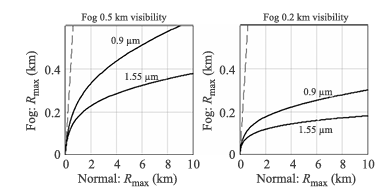
\includegraphics[width=0.5\linewidth]{figures/Range_Degradation_Fog.png}
    \caption{Range degradation curves for fog conditions}
    \label{fig:placeholder}
\end{figure}

Additionally it is to be noted, that the absorption coefficient in water, is significantly higher for 1550nm wavelengths, than for 905nm or 850nm wavelengths. For 905nm the absorption coeffiecient $\gamma_{905nm} = 0.075cm^{-1}$, while for 1550 $\gamma_{1550} = 10.8cm^{-1}$ \cite{wojtanowski_comparison_2014}. That means the absorption coefficient of 1550nm wavelength signals is a factor 144 larger than those of 905nm. This leads to a significant decrease in range for 1550nm LiDAR sensors.
In these plots the x-axis corresponds to the original maximum range, while the y-axis corresponds to the maximum range under the conditions written above  the plot \cite{wojtanowski_comparison_2014}. 


\subsection{Rain}

When water falls back to the ground after condensating, it is referred to as percipation. Its intensity, which is measured in millimeters per hour, is defined by the droplets size and distribution. When the electromagnetic signals of the LiDAR propagte through the percipated medium, it is affected by Mie Scattering \cite{vargas_overview_2021}. The maximum diameter of a droplet, is 6mm. If a droplet were to be larger than that, it would explode into smaller fragments due to friction forces acting on the droplet \cite{hadj-bachir_lidar_2019}. Mie Scattering will affect the propagation of the electromagnetic signal in two way. It will cause attenuation due to the absorption of the electromagnetic energy by the droplet. Additonally the droplet can backscatter the signals, which can then cause false positive points. 
As LiDAR mostly transmitts 905nm or 1550nm wavelengths, it will be affected by Mie Scattering which causes significant degradation. As explained for fog, 1550nm waves have an absorption coefficient which is a factor 144 larger than that of 905nm waves \cite{wojtanowski_comparison_2014}. This also highlights, that the LiDAR behaviour in adverse weather is also very dependant on which specific LiDAR sensor is being used.  
In figure ~{2.4} this bahaviour for rain is highlighted \cite{wojtanowski_comparison_2014}. 

\begin{figure}[htbp]
    \centering
    \begin{subfigure}[t]{0.48\linewidth}
        \centering
        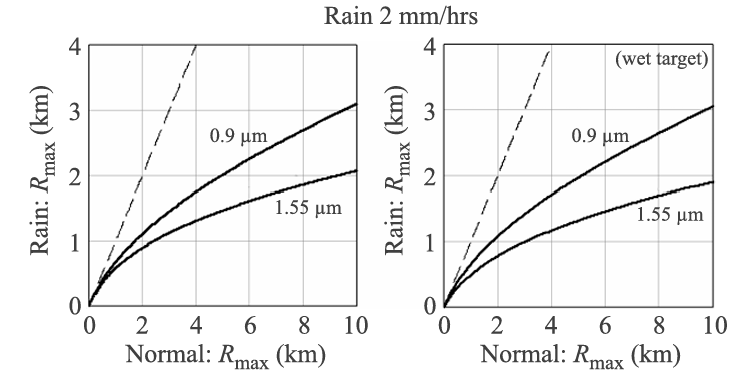
\includegraphics[width=\linewidth]{figures/Range_Reduciton_Rain_2mm.png}
        \caption{Rain intensity: 2 mm/h}
        \label{fig:rain2mm}
    \end{subfigure}
    \hfill
    \begin{subfigure}[t]{0.48\linewidth}
        \centering
        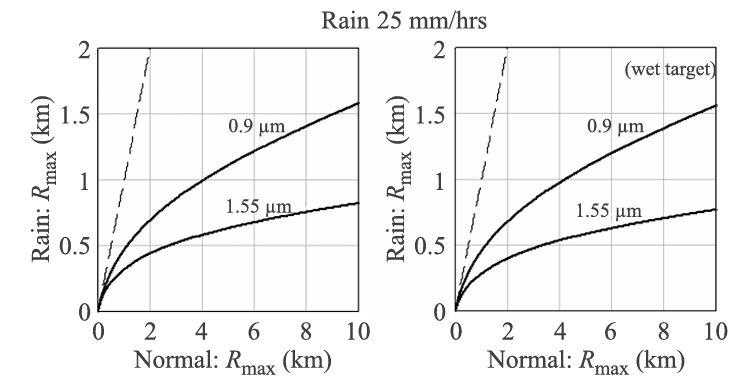
\includegraphics[width=\linewidth]{figures/Range_Reduciton_Rain_25mm.png}
        \caption{Rain intensity: 25 mm/h}
        \label{fig:rain25mm}
    \end{subfigure}
    \caption{Range degradation curves under rain conditions}
    \label{fig:range_degradation_rain}
\end{figure}

It can be seen, that the maximum range $R_{max}$ drops significantly for both 2 millimeter per hour as well as 25 millimeter per hour rain. Even with the lighter configuration, the range for the 905nm LiDAR sensor is only 30\% of it's clear weather range and due to higher absorption it is even less for the 1550nm LiDAR. With stronger rain of 25 millimeters per hour, the maximum range $R_{max}$ drops to only 15\% of its clear weatherperformance. For closer objects, the performance is better but still is only around 50\% for 905nm in light rain and about 25\% for 905nm in strong rain. For both situations it even degrades a little bit further if the target itself is also wet. 

Nevertheless, when compared to figure ~(2.3), which illustrates the range depreciation for fog, it becomes apparent, that the range is still significantly higher for rain, than it is for fog. 
In fog the number of droplet per $cm^3$ is about 100, while rain only has about 0.001 droplet per $cm^3$.
Thats is about a factor $10^5$ \cite{teufel_simulating_2022}. Therefore, there are $10^5$ fewer droplets blocking the LiDAR's beam, reducing the probability of deletion and, consequently, explaining the higher visibility in rain compared to fog. 

In addition to the point deletion, there is backscattering, geometric distortion, and ranging error. %FIND SOURCE.  
Backscattering occurs when LiDAR light pulses encounter water particles, such as raindrops, which prevent the light from fully penetrating the intended target. Instead of passing through these particles, the light is reflected and continues to create a spurious peak in the received signal power at an incorrect position \cite{hahner_fog_2021} This effect is significantly more prevalent in rain than in fog. This has been demonstrated by calculating the backscattering coefficient $\beta_{back}$ and the received power using equation ~(x). 

\begin{equation}
    Backscattering equation here 
\end{equation}

It can be seen that the backscattering coefficient and the received power $P(R)$ are both dependent on the droplet size $D$, underlining the importance of backscattering in rain. As the rain rate rises, the hit probability also rises, making it also dependant on the rain rate \cite{haider_methodology_2023}. 



%%%%Talk abouot Intensity as well here%%%%

\section{Current approaches to modeling \& Validation LiDAR Point Cloud Faults Faults}


Recent literature suggests, that rain is mostly modeled using physical simulators and techniques such as ray tracing, while fog is often modeled in a probabilistic way. This is due to the high number of droplets in fog, which makes it computationally very expensive to model \cite{teufel_simulating_2022}.  

In the following, Table 2.3 is introduced, which presents the most important authors, the effects they addressed, and their validation approaches. 

%%%%%Adjust this to what im actually referencing and compare to source. Currently not correct. %%%%%%%%%
%
% \begin{table}[t]
% \centering
% \caption{Overview of LiDAR weather-related studies}
% \label{tab:weather_lidar}
% \renewcommand{\arraystretch}{1.15}
% \begin{tabularx}{\textwidth}{@{}p{3.2cm} p{3.2cm} p{5.0cm} p{3.0cm}@{}}
% \toprule
% \textbf{Authors} &
% \textbf{Weather Phenomena} &
% \textbf{Observed Effects} &
% \textbf{Validation} \\
% \midrule
%
% Goodin et al.~\cite{goodin} &
% Rain &
% Signal attenuation, false negatives, ranging error, reduced max. range &
% Simulation \\
% \midrule
%
% Wojtanowski et al.~\cite{wojtanowski} &
% Rain, fog, aerosols &
% Signal attenuation, reflectivity changes, range degradation &
% Simulation \\
% \midrule
%
% Rasshofer et al.~\cite{rasshofer} &
% Rain, fog, snow &
% Signal attenuation, range degradation &
% Simulation + qualitative fog measurements \\
% \midrule
%
% Byeon et al.~\cite{byeon} &
% Rain &
% Signal attenuation &
% Simulation \\
% \midrule
%
% Li et al.~\cite{li} &
% Rain, fog, snow, haze &
% Signal attenuation &
% Simulation \\
% \midrule
%
% Zhao et al.~\cite{zhao} &
% Rain, fog, snow, haze &
% Signal attenuation, false positives &
% Quantitative (rain) \\
% \midrule
%
% Guo et al.~\cite{guo} &
% Rain &
% Signal attenuation &
% Qualitative \\
% \midrule
%
% Hasirlioglu et al.~\cite{hasiroglu} &
% Rain &
% Signal attenuation, false positives &
% Quantitative \\
% \midrule
%
% Berk et al.~\cite{berk} &
% Rain &
% Signal attenuation, false positives &
% Simulation \\
% \midrule
%
% Espineira et al.~\cite{espineira} &
% Rain &
% Signal attenuation, false positives &
% Simulation \\
% \midrule
%
% Kilic et al.~\cite{kilic} &
% Rain, fog, snow &
% Signal attenuation, false positives &
% Quantitative \\
% \midrule
%
% Hahner et al.~\cite{hahner} &
% Fog &
% Signal attenuation, false positives &
% Quantitative \\
% \midrule
%
% Haider et al.~\cite{haider_methodology_2023} &
% Rain, fog &
% Signal attenuation, SNR, false pos./neg., ranging error &
% Qualitative \\
%
% \bottomrule
% \end{tabularx}
% \end{table}


It becomes apparent that fog but especially rain are the most researched topics in the realm of fault injection. The covered effects also give some insight into what to focus on. Signal attenuation and false positives are the most commonly covered effects. When comparing this to the physical effect in the previous section, it becomes apparent why this is the case. Additional effects covered in the current literature are range errors $d_{error}$, range degradation, and SNR. In the following, these effects will be explained for fog and rain, focusing on the most important ones. We need to build a simple yet effective fault injection tool.

The validation approach can only be divided into two main approaches, one being simulaiton results and the other being comparison to real measurements. 

In the following subsections, fog and rain modelling as well as the validation of faults will be discussed. 



\subsection{Fog Modelling}
In the previous section the physical effects of weather on the laser beam of a LiDAR sensor were discussed. To accurately model fog, it is important to understand the effect this degradation has on the point cloud so it can be simulated. 

The effects of fog on the point cloud can be divided into the following three categories: 

Noise Augmentation \cite{teufel_enhancing_2023}: 
This effect mimics the formation of false points due to backscattering. This means that the laser beam is reflected by the droplet, with an intensity detectable by the photodetector. 
Drop Out \cite{teufel_enhancing_2023}: 
Dropout imitates the loss of points due to attenuation of the signal. This effect is the main cause for the immense range reduction observed in Figure 2.4. 
Intensity \cite{teufel_enhancing_2023}: 
Due to reflections from laser beams in the fog, the intensity degrades significantly. This causes weaker return signals and 
Distance Error \cite{heinzler_weather_2019}
 The ranging error $d_{error}$ is caused by the misalignment of the LiDAR rays due to reflection from the raindrops, leading to a shift in the peak location and distorting the final position of the points in the point cloud. These errors are fairly small for fog and increase as the droplet size increases and the visibility decreases. 
Measurements conducted by the KIT have shown that under foggy conditions with a visibility of 300 meters, the distance error per point reaches around 1.2cm. The maximum distance error is said to be below 2cm \cite{haider_methodology_2023}.
Teufel et al. suggest a probabilistic fog model, due to the high amount of droplets per $cm^3$ and how computationally expensive it would be to model physically. 
This approach defines the probability that a point is modified as $p_{modify}$, the probability that a point is deleted due to backscattering, given it has been selected to be modified as $p_{deleted}$ ,and the probability that a point is moved due to backscattering as $p_{move}$. If a point is selected for movement, it is moved closer to the sensor, simulating the backscattering behaviour described above \cite{teufel_simulating_2022}. Teufel et al. imply a dependence on the visibility under fog, similar to what has been described earlier. In this approach, the visibility is the parameter that can be adjusted to set the severity of the fault. 
Additionally, Teufel et al. suggest adjusting the intensity of the unaltered points with respect to the distance: $I(d)$ \cite{teufel_simulating_2022}. 
These probabilities are then sampled from a Bernoulli distribution, yielding a binary output. When sampling a probability, the output is either $1$ with a probability of $p_{modify}$ or 0 with a probability of $1-p_{modify}$. Based on these results, points in the point clouds are then chosen for modification, deletion, and backscattering. 
The equations in Teufel's approach are tuned using the Chafer metric using the DENSE dataset \cite{bijelic_seeing_2019}. This dataset is a novel dataset that includes point clouds that have been distorted in a rain and fog chamber. 

Based on the approach above, it is then possible to modify an existing point cloud.

Another approach discussed in the literature is a physical approach, which is more complex and also computationally more expensive. This approach moves beyond data augmentation by attempting to replicate the interaction between the laser pulses and atmospheric particles in the signal domain. It uses a decision logic based on returned power and Mie Scattering, as explained earlier \cite{hahner_fog_2021}. 
Haider et al. suggest that, in addition to the signal attenuation and backscattering implemented by Hahner et al. or Teufel et al., it is also important to consider the signal-to-noise ratio (SNR)caused by rain or fog droplets. This then leads to a point cloud error, described as $d_{error}$ \cite{haider_methodology_2023}. Figure ~(2.6) from Teufel et al. illustrates the modification by the probabilistic fog model: 

\begin{figure}[htbp]
    \centering
    \begin{subfigure}[t]{0.48\linewidth}
        \centering
        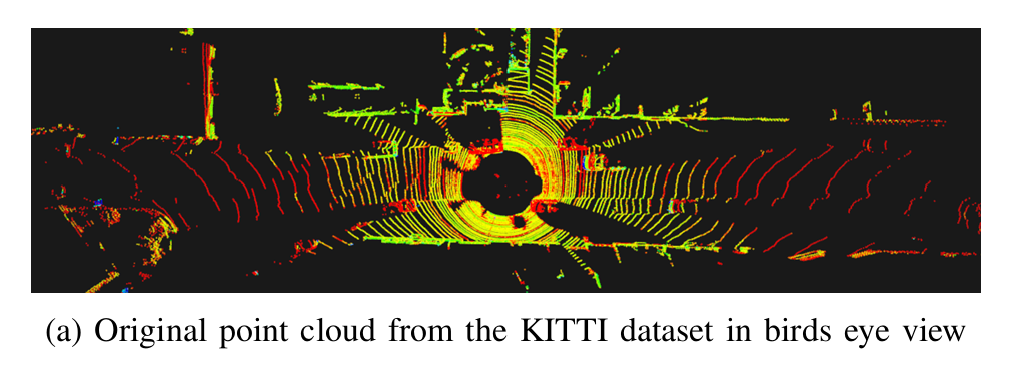
\includegraphics[width=\linewidth]{figures/Original_Visbility_Clear.png}
        \caption{Visbility: Clear, without any filter.}
        \label{fig:rain2mm}
    \end{subfigure}
    \hfill
    \begin{subfigure}[t]{0.48\linewidth}
        \centering
        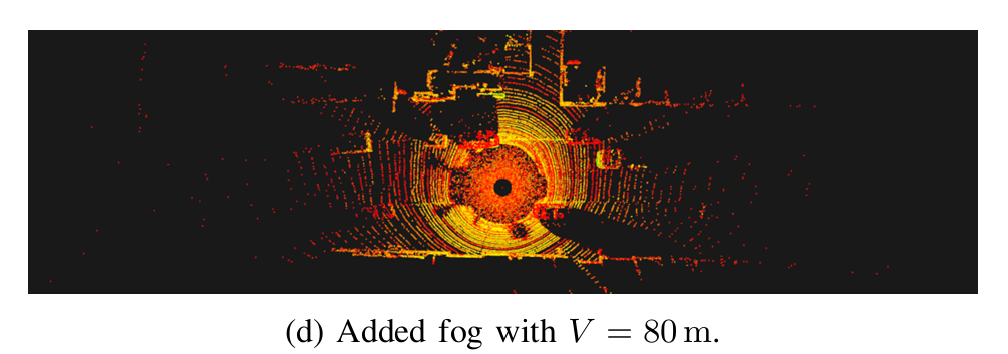
\includegraphics[width=\linewidth]{figures/Fog_Visbility_80m.png}
        \caption{Visbility: 80m visibility}
        \label{fig:rain25mm}
    \end{subfigure}
    \caption{Localization scans in clear and foggy conditions.}
    \label{fig:range_degradation_rain}
\end{figure}

\subsection{Rain Modelling}
When modelling rain faults, we need to undertake similar modifications on the LiDAR point cloud as in fog approaches. 
The most important ones are: 

Point Deletion: Deletion of points due to attenuation of signal intensity. This effect is not prevalent in rain as it is in fog. 

Backscattering: Backscattering due to interaction between the laser beam and the droplet, causing a false positive point within the point cloud.

Intensity: Intensity degradation due to attenuation of the singal. These signal attenuations weren't severe enough for deletion.

Geometric Distortion: Due to penetration of the droplets, the LiDAR beams are also distorted. Due to the large size of rain drops comapred to fog, this effect is highly relevant for rain. 

In comparison to fog, rain models have not been probabilistically modeled with the goal of modifying a point cloud. Instead most rain simulations use physical simulations to create a new distorted point cloud \cite{haider_methodology_2023} \cite{hasirlioglu_model-based_2018}. 

These model rain as a collection of individual water droplets, which are usually characterized by their size, spatial distribution, and interaction with the emitted laser beams \cite{haider_methodology_2023}.
These droplet sizes vary significantly and in natural rain the maximum diameter is around 6mm, as discussed earlier \cite{earlier}.
Fall speeds can also vary and range  from 0.1 $m/s$ to more than 9 $m/s$.
parameters required by the simulation to model the range vary \cite{FIND}. Physical models therefore use multiple input parameters to create the simulation. The Marshall Palmer Drop Size Distribution, physical dynamics such as the terminal velocity and gravity, drop concentration or sensor specific parameters \cite{zhao_method_2021} \cite{haider_methodology_2023}. 
These methods then create new, distorted point clouds by simulating the interaction between laser pulses and water particals on signal level. Two primary ways of doing this are through ray tracing or signal domain transformations. 
Performing ray tracing was implemented by for example both Teufel et al and Hasirlioglu et al. This method simulates rain as a 3D volume filled with physical spheres \cite{teufel_simulating_2022}. This approach creates a noise filter consisting of spherical drops in the sensor's field of view. It then traces multiple diverging rays for every single point to account for beam divergence \cite{teufel_simulating_2022}. Some papers then evaluate the hit ratio of rays from a point with the noise filter. If the hit ratio is then above a certain threshold the point is modified \cite{hasirlioglu_model-based_2018}. Others use the intensity as a guiding principle for deletion \cite{kilic_lidar_2021}. This then creates a new point cloud based on the interaction of the raindrops. These models then output a spatially relistic point cloud. 

The other approach uses Mie Scattering theory to calculate extinction coefficients for both signal loss and backscattering. These then compare the emitted power and delete if it is below a certain threshold. Although this paper aims to modify an existing point cloud, this is very helpful to understand the physical effects happening in rain and what exactly has to be modified \cite{haider_methodology_2023}. 
Nevertheless these models are very computationally expensive to model. 

A third approach is a stochastic model, also referred to as point cloud modification \cite {teufel_enhancing_2023}. This model considers noise augmentation and drop out to model the rain effects \cite{teufel_enhancing_2023}. The benefit of such a model is that it does not require computationally expensive methods such as ray tracing. The downside is that the rain models themselves are less accurate than a physical simulation. These don't account for hardware or geometric distortion. This approach has been used in the literature to train object detection algorithms and, therefore, might not be a good choice for a rain model. 

In comparison to fog, it becomes apparent that there is no ideal solution to the approach this thesis follows. There are many physical models that create new point clouds and are very computationally expensive. The other option is a simple and data-driven approach that does not consider LiDAR physics at all. 

Nevertheless, it is important to realize that the measured effects discussed earlier are very similar to fog. The main difference is the way they are weighted. While for fog deletion is the primary source for distortion, this is not the case for rain. For rain backscattering and geometric distrotion seem to be more impactful. 

\subsection{Comparison of Fog impact on point cloud to Rain impact on Point Cloud }

As we have seen the effects that are modeled in the physical simulations for rain are quite similar to those in the fog simulation from Teufel et al. The exact difference can be seen in Table ~(2.4). Translating this into the mechanisms for point cloud modification discussed earlier. It can be seen that the extinction coefficient for rain is significantly lower than for fog \cite{wojtanowski_comparison_2014}. This makes point deletion significantly more prevalent for fog. An object detection test run showed, that at 98mm/h rain the detection rate dropped to about 82.3\%, while fog couldnt detect it anymore.

Backscattering tells a similar story

Ranging Error on the other hand seems to be signifcantly more intense, which can be explained due to the large droplet \cite{haider_methodology_2023}

\begin{table}[h!]
\centering
\caption{Impact of Adverse Weather Conditions on Sensor Performance}
\label{tab:weather_comparison}
\begin{tabular}{lcc}
\hline
\textbf{Parameter} & \textbf{Rain (Heavy: 98 mm/h)} & \textbf{Fog (Dense: $<100$ m Visibility)} \\
\hline
Droplet Diameter ($D$) 
& Avg. $1$ mm (up to $6$ mm) 
& $0.1~\mu$m to $20~\mu$m \\

Particle Density 
& $\sim 10^{3}$ droplets/m$^{3}$ 
& $\sim 10^{6}$ droplets/m$^{3}$ \\

Detection Rate (DR) 
& $\sim 82.3\%$ (at 20 m) 
& Significantly lower than rain \\

False Detection Rate (FDR) 
& $\sim 22.7\%$ 
& $300\%$ to $500\%$ \\

Distance Error ($d_{\text{error}}$) 
& Up to $4.9$ cm 
& Less than $2.0$ cm \\

Signal Attenuation ($\sigma_{\text{ext}}$) 
& Lower overall attenuation 
& Up to $9.2$ dB (at 50 m visibility) \\

Primary Failure Mode 
& Geometric distortion (misalignment) 
& Signal loss (attenuation) \\
\hline
\end{tabular}
\end{table}

--> Check more Literature for better data on this. 

Takeaways: 

- Point Deletion and Detection Rate: A LiDAR can still accurately detect an object under strong rain, while it cannot do the same for strong fog. Due to higher amount of droplets

- Backscattering and False Deteciton Rate: 
\section{Current Localizations algorithms}
The goal is to evaluate how our localization reacts to certain weather faults and their respective severity. In order to understand which parameters to evaluate and how to interpret them, it is cruical to understand what localization is and how it works. 

In order to accurately determine the vehicle's position and understand its surroundings, the AV needs a map of its surroundings as well as its specific position within that map. While Mapping uses the sensors' data to create a map of its surroundings, localization uses the sensors' data to determine its own position within a map.



A common method for localization is odometry. It determines the relative change in position in between two points in time. Algorithms usually use multiple sensors to accurately determine its position. 
For LiDAR this is the primary localization method. 
As this thesis focuses primarily on LiDAR faults for localization, in the following the operating principle of localization with LiDAR data will be explained. 
Relative localization through odometry uses a Scan matching principle. This estimates the relative pose change by analyzing two consecutive LiDAR scans. The algorithm iteratively aligns the second scan with respect to the first until a maximum geometric correspondence between both scans is achieved. A representative example of such an approach is the Iterative Closest Point (ICP) algorithm.

Such algorithms can then determine the exact position and orientation of a vehicle in between the scans. This is done by calculating the rotation and the translation between two consecutive scans and searching for similarities. 

Some scan matching algorithms that are commonly used today are: 
\begin{itemize}
    \item Iterative Closest Point (ICP)
    \item Normal Distributions Transform (NDT)
    \item Point-to-Line ICP
    \item Correlative Scan Matching (CSM)
\end{itemize}


\subsection{Validation of Faults}

After discussing both physical and probabilistic approaches, the question arises: how can they be validated? The two primary approaches are comparing the results to real-world or test environment data and comparing the simulated results to a dataset that was recorded in fog or other simulations. 
The first approach is the most meaningful, as it allows a direct comparison against real-world behaviour. The downside is the high cost to acquire the data. 
For example, Haider et al. set up an experiment inside a fog chamber and compared their simulated results against the real-world results they received from measurements inside the chamber \cite{haider_methodology_2023}. This is a very accurate approach to verify the accuracy of the simulation, as the rain rate, humidity and the visibility can be adjust or kept constant, making for a good comparison. Haider then evaluated the signals at the time-domain and point-cloud levels. At the time-domain level, the extinction coefficient and SNR are considered. On the point cloud level, the detection rate, false detection rate as well as the distance error $d_{error}$ are considered \cite{haider_methodology_2023}. 

An additional performance indicator in the point cloud domain is the number of points in the point clouds and the intensity of each point \cite{kim_empirical_2023}.
This is also a metric used by other papers, such as \cite{alavi_quantifying_2025}
, and validates the number of points as a good metric. This paper then also reviews the mean and the standard deviation across multiple measurements and compares it to other simulations\cite{alavi_quantifying_2025}.
From the amount of points, it is then also possible to calculate the Point Survival Rate (PSR) or the False Positive Rate (FPR) \cite{haider_methodology_2023}.
This gives a good understanding of signal attenuation in regard to precipitation and fog.

A good metric for comparing these performance indicators across measurements is the Mean Absolute Percentage Error (MAPE), as shown in Equation (2.4) \cite{haider_methodology_2023}. 
\begin{equation}
\mathrm{MAPE} = \frac{1}{n} \sum_{t=1}^{n} 
\left| \frac{V(t) - P(t)}{V(t)} \right| \cdot 100
\end{equation}
In this equation $V(t)$ is the actual value at time step $t$
$P(t)$ is the predicted value at time step $t$
and $n$ represents the number of evaluation periods \cite{noauthor_mape_nodate}. 

Equally important is the evaluation of the impact LiDAR faults have on the localization. For localization algorithms, it is important to evaluate both their relative and their absolute error. Therefore the absolute position error (APE) as well as the relative position error (RPE) have to be taken into consideration. These performance indicators are calculated by aligning the  trajectories of the localization algorithm with the ground truth trajectory \cite{morelli_deep_2025}. 

These errors are then summarized using the Root Mean Squared Error (RMSE) shown in Equation ~(2.6). 

\begin{equation}
\mathrm{RMSE} = \sqrt{\frac{1}{N} \sum_{i=1}^{N} e_i^2}
\end{equation}

This then sums up the relative errors and creates a weighted metric that is a good indicator of how well the algorithm performs. 
\section{Research Gap }

Table~ ~(2.3) shows that there is significant research on weather simulation and their impact on LiDAR sensors. 
Additionally, various localization algorithms have been developed and tested. 
Nev,ertheless it has become apparent how badly autonomous vehicles perform in adverse weather. To better understand the localization and define the exact operational desing domain it is very important to understand exactly what impact weather has on the localization. 

An in-depth literature review has shown that there is research focusing on weather simulations of LiDAR measurements and also some papers that analyze the effect this has on object detection. What hasn't been done yet is to evaluate the effect these conditions have on the localization algorithm and quantify what impact each weather scenario has. Real-world tests have been found to be unfeasible for this type of development, as they would be too costly initially and would require too much driving as well as validation of each adjustment to the AV' system\cite{kalra_driving_2016}. This is why developing a simulation tool, that can modify existing, clear point clouds and directly compute the localization is essential to advance AV safety. 

The literature research on weather simulations showed that there is a lot of literature on simulating actual weather scenarios and the interaction of LiDAR rays with the droplets, but not on point cloud modification, at least for rain. As fog has a significantly larger amount of droplets per $cm^3$ it has been simulated probabilistically, which can easily be sampled to modify an existing, clean point cloud \cite{teufel_simulating_2022}. However, rain hasnt been simulated in this way. Most rain simulations are either physical simulations, which trace the interaction of each ray with each rain drop creating an entirely new point cloud or not physical at all, only sampling from distributions. Aside from the computational power it requires to run these physical simulations, it also requires advanced optics knowledge that would go beyond the scope of this work. As the goal of this thesis is to create a weather framework, validate it and evaluate the impact it has on a localization algorithm it will define a novel approach to probabilistically modify clear point clouds to mirror the effects rain has on LiDAR measurements. In order to do this, it is important to analyze the physical simulations and the respective results in order to accuretly model them. 












